\begin{figure}[h]
\centering
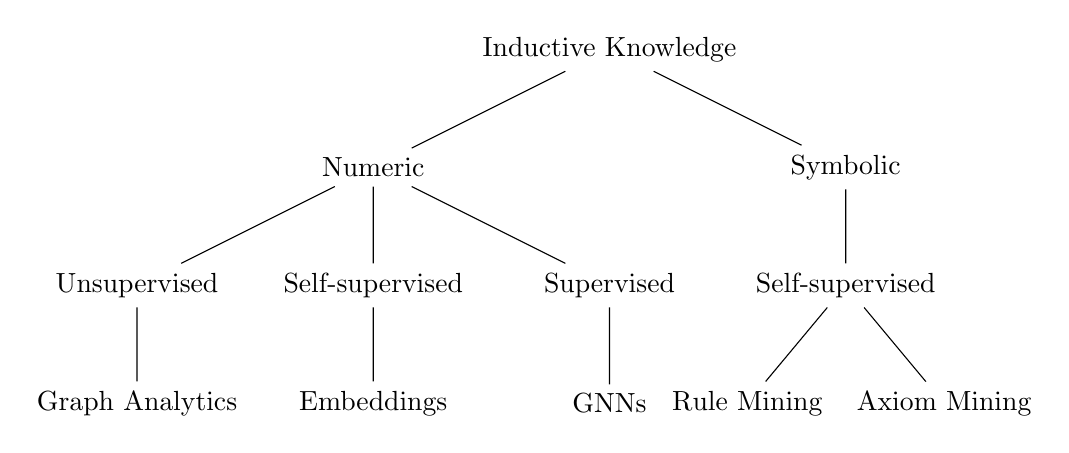
\begin{tikzpicture}[level distance=1.5cm, sibling distance=2.5cm]
\tikzset{
    every node/.style={align=center},
    level 1/.style={sibling distance=6cm},
    level 2/.style={sibling distance=3cm},
    level 3/.style={sibling distance=2.5cm}
}

\node {Inductive Knowledge}
    child {
        node {Numeric}
        child {
            node {Unsupervised}
            child {node {Graph Analytics}}
        }
        child {
            node {Self-supervised}
            child {node {Embeddings}}
        }
        child {
            node {Supervised}
            child {node {GNNs}}
        }
    }
    child {
        node {Symbolic}
        child {
            node {Self-supervised}
            child {node {Rule Mining}}
            child {node {Axiom Mining}}
        }
    };
\end{tikzpicture}

\caption{Overview of popular techniques for extracting inductive knowledge from a knowledge graph \parencite{hogan2021knowledge}.}
\label{fig:inductive_kg}
\end{figure}